\documentclass{article}
\usepackage{graphicx} % Required for inserting images
\usepackage{CJKutf8}
\usepackage{amsthm}
\usepackage{mdframed}
\usepackage{float}

\title{hw11}
\author{110201534}
\date{}

\begin{document}
\begin{CJK*}{UTF8}{bkai}
\maketitle

\section*{problem 1}
\subsection*{1}T, suppose the contrary that exist a planar graph G with there is a subgraph is not planar, means that for every drawing of this subgraph, must exist crossing in the subgraph, it implies that the graph is not a planar, then we get a contradiction.
\subsection*{2}F, disprove this statement with a counter-example
\begin{figure}[H]
    \centering
    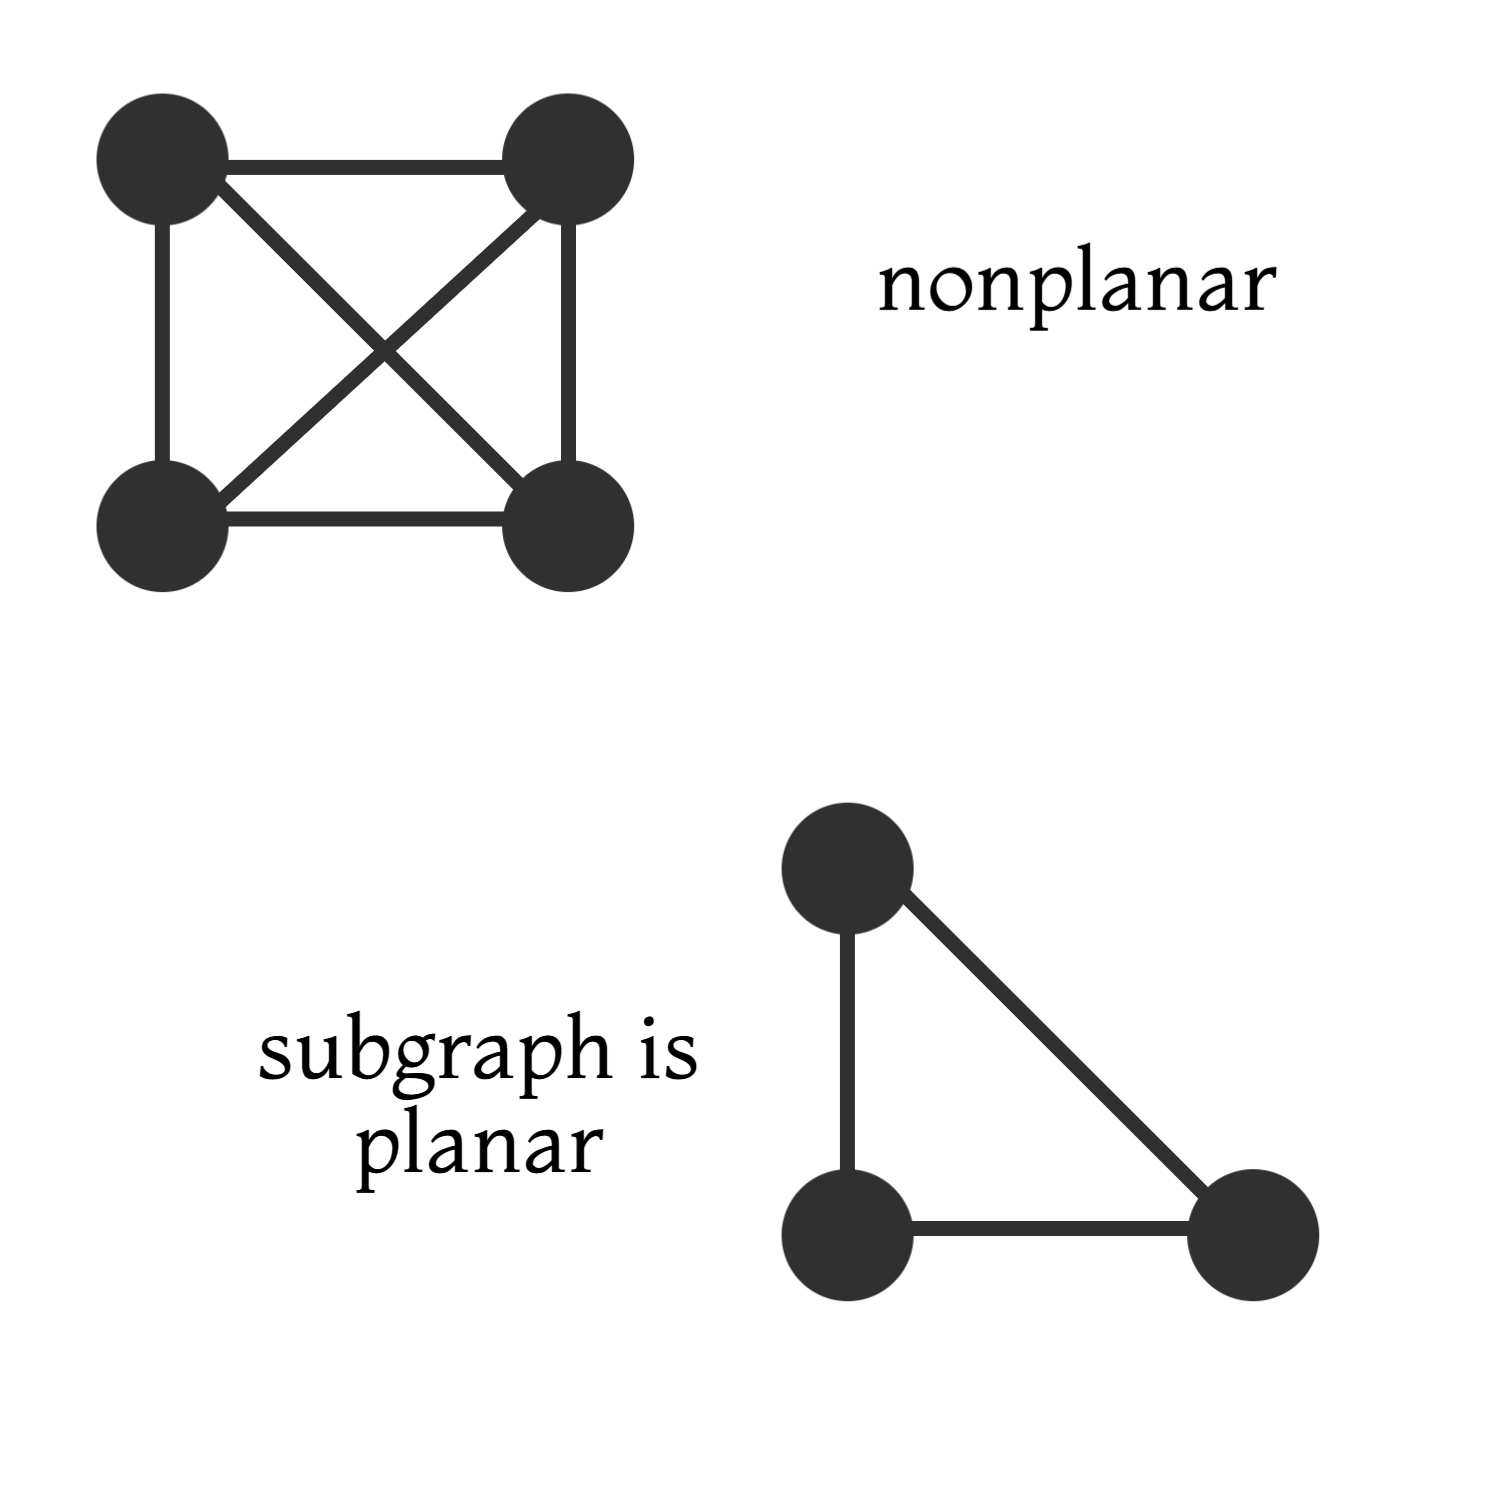
\includegraphics[scale = 0.1]{counterexample.jpg}
    \caption{counter-example}
\end{figure}
\section*{problem 2}
suppose the order of G is n, the size of G is e and the number of face of G is f, since G is a triangulation, 
by Euler's formula, we have $n+f-e=2 \Rightarrow n + f - (3n-6)=2 \Rightarrow f = 2n-4$

and $\sum_{i} l(F_{i}) = 3f = 6n-12 = 2e(G) = \sum_{v \in V(G)} deg(v)$

so we can get the result : $\sum_{i} 6n_{i} - \sum_{i} in_{i}$ = 6n - (sum of degree) = 6n - (6n-12) = 12

\section*{problem 3}

%%% note


%%% end of note

\end{CJK*}
\end{document}
